\documentclass[aspectratio=169]{beamer}
\usetheme{Madrid}
\usecolortheme{default}
\usepackage{graphicx}
\usepackage{booktabs}
\usepackage{tikz}
\usepackage{hyperref}

\title[FloodEye]{FloodEye: Real-time Flood Alert \& Water Level Monitoring}
\subtitle{IoT and Machine Learning based Early Warning System}
\author{Project Team}
\date{\today}

\begin{document}

\begin{frame}
  \titlepage
  \vspace{-1cm}
  \begin{center}
    
\includegraphics[height=1.5cm]{../public/logotih.png} \hspace{1cm}
    
\includegraphics[height=1.5cm]{../public/iitlogo.png}
  \end{center}
\end{frame}

\begin{frame}{Agenda}
  \tableofcontents
\end{frame}

\section{Project Overview \& Motivation}

\begin{frame}{Project Overview}
  \begin{itemize}
    \item \textbf{FloodEye} is a highly responsive Progressive Web Application (PWA).
    \item Designed to visualise real-time water level data and environmental conditions.
    \item Uses an ESP32 microcontroller and multiple sensors (BMP180, DHT11, HC-SR04).
    \item Combines IoT telemetry, a glassmorphism UI, interactive maps, and ML.
    \item Aims to provide an early warning system for flood-prone areas.
  \end{itemize}
\end{frame}

\begin{frame}{Motivation}
  \begin{itemize}
    \item Floods cause devastating loss of life and property globally.
    \item Traditional monitoring systems are often expensive, slow, or inaccessible to the public.
    \item Need for a low-cost, open-source, and real-time monitoring solution.
    \item Integration of modern web technologies (Next.js) with edge IoT and browser-based AI (TensorFlow.js) bridges the gap between hardware and accessible user interfaces.
  \end{itemize}
\end{frame}

\begin{frame}{Key Value Proposition}
  \begin{itemize}
    \item \textbf{Low Cost:} Utilises off-the-shelf components (ESP32, ultrasonic sensors).
    \item \textbf{Real-Time:} 15-second refresh interval for live telemetry.
    \item \textbf{Predictive:} 4-hour advanced flood warning using an in-browser 1D-CNN + BiLSTM + Attention model.
    \item \textbf{Accessible:} PWA allows installation on any mobile device or desktop.
  \end{itemize}
\end{frame}

\section{Problem Statement \& Objectives}

\begin{frame}{Problem Statement}
  \begin{itemize}
    \item Communities in flood-prone regions lack actionable, real-time data regarding local river water levels.
    \item Existing weather apps provide regional rainfall forecasts but lack micro-local hydrological data.
    \item Hardware telemetry is often disconnected from modern, user-friendly predictive analytics.
    \item \textbf{Challenge:} Build a reliable, low-latency, end-to-end system spanning from physical water sensors to a public-facing predictive dashboard.
  \end{itemize}
\end{frame}

\begin{frame}{Primary Objectives}
  \begin{itemize}
    \item \textbf{Hardware Data Acquisition:} Continuously read water distance, temperature, humidity, and atmospheric pressure.
    \item \textbf{Cloud Integration:} Reliably transmit telemetry data to a cloud platform (ThingSpeak).
    \item \textbf{Full-Stack Dashboard:} Develop a Next.js application to visualise live and historical data.
    \item \textbf{Predictive AI:} Train and deploy an ML model to forecast water levels 4 hours into the future.
  \end{itemize}
\end{frame}

\begin{frame}{Secondary Objectives}
  \begin{itemize}
    \item \textbf{Smart Alerts:} Implement a highly configurable alert engine with cooldowns and push notifications.
    \item \textbf{Offline Resilience:} Ensure the dashboard remains functional (showing cached data) even if the IoT node goes offline.
    \item \textbf{Data Export:} Allow researchers to download historical data (CSV/PDF).
    \item \textbf{Role-Based Access:} Secure administrative controls for threshold configuration.
  \end{itemize}
\end{frame}

\section{System Architecture \& Workflow}

\begin{frame}{System Architecture: Three-Tier Model}
  \begin{itemize}
    \item \textbf{Hardware Layer:} ESP32 DevKit + Sensors. Uploads to ThingSpeak via HTTP REST.
    \item \textbf{Backend Layer:} Next.js Route Handlers fetch data, apply request coalescing, and perform caching.
    \item \textbf{Frontend Layer:} React/Next.js UI. Renders cards, charts, maps, and runs TF.js ML inference entirely client-side.
  \end{itemize}
\end{frame}

\begin{frame}{Hardware Workflow}
  \begin{itemize}
    \item ESP32 powers on and initialises sensors via I$^2$C and digital pins.
    \item Main loop reads water level (ultrasonic), temperature/humidity (DHT11), and pressure/altitude (BMP180).
    \item Packages data into an HTTP POST payload.
    \item Transmits to ThingSpeak every 15 seconds.
    \item Features exponential backoff for Wi-Fi reconnection in case of failure.
  \end{itemize}
\end{frame}

\begin{frame}{Backend Data Flow}
  \begin{itemize}
    \item Client polls \texttt{/api/sensors} every 15 seconds.
    \item Serverless function checks in-memory cache (singleton pattern).
    \item If cache is fresh ($< 14$s), returns immediately.
    \item If stale, fetches from ThingSpeak Cloud.
    \item Coalescing ensures concurrent requests share a single ThingSpeak API call, preventing rate limits.
  \end{itemize}
\end{frame}

\begin{frame}{Frontend \& ML Workflow}
  \begin{itemize}
    \item Dashboard mounts and hydrates state from \texttt{localStorage} (offline resilience).
    \item \texttt{TelemetryProvider} updates global state with new readings.
    \item Smart Alert engine evaluates thresholds (e.g., RAPID\_WATER\_RISE).
    \item \texttt{useFloodPrediction} hook parses the last 48 readings.
    \item Features are engineered and passed to TensorFlow.js model.
    \item 4-hour forecast is rendered on the UI.
  \end{itemize}
\end{frame}

\section{Technology Stack \& Hardware Components}

\begin{frame}{Hardware Components}
  \begin{itemize}
    \item \textbf{Microcontroller:} ESP32 DevKit V1 (Wi-Fi enabled, dual-core).
    \item \textbf{Water Level Sensor:} HC-SR04 Ultrasonic Sensor (measures distance to water surface).
    \item \textbf{Atmospheric Sensor:} BMP180 (measures barometric pressure and altitude via I$^2$C).
    \item \textbf{Environmental Sensor:} DHT11 (measures ambient temperature and relative humidity).
    \item \textbf{Power:} 5V USB power supply / Battery pack.
  \end{itemize}
\end{frame}

\begin{frame}{Software Technology Stack: Frontend}
  \begin{itemize}
    \item \textbf{Framework:} Next.js 16 (App Router) with React 19.
    \item \textbf{Styling:} Tailwind CSS v4 + Framer Motion (glassmorphism \& animations).
    \item \textbf{Charts:} Recharts for responsive, interactive SVG time-series analytics.
    \item \textbf{Map:} MapLibre GL JS + MapTiler for live node location overlays.
    \item \textbf{PWA:} \texttt{next-pwa} for service worker generation and offline caching.
  \end{itemize}
\end{frame}

\begin{frame}{Software Technology Stack: Backend \& ML}
  \begin{itemize}
    \item \textbf{Backend API:} Next.js Serverless Route Handlers (\texttt{/api/sensors}, \texttt{/api/history}).
    \item \textbf{IoT Cloud:} ThingSpeak (MathWorks) for telemetry storage.
    \item \textbf{Machine Learning (Training):} Python, TensorFlow/Keras, Pandas, Scikit-learn (Google Colab).
    \item \textbf{Machine Learning (Inference):} TensorFlow.js running in the browser (Zero server cost).
  \end{itemize}
\end{frame}

\section{UI Screens \& Features}

\begin{frame}{Landing Page \& Scrollytelling}
  \begin{itemize}
    \item An immersive, GSAP-powered root page (\texttt{/}).
    \item Features a background slideshow of flood monitoring imagery.
    \item ScrollTrigger and Lenis provide smooth scroll animations.
    \item Introduces the project, team members, and core technologies.
    \item Direct CTA (Call to Action) to open the Live Dashboard.
  \end{itemize}
\end{frame}

\begin{frame}{Main Dashboard}
  \begin{columns}
    \begin{column}{0.5\textwidth}
      \begin{itemize}
        \item Five real-time sensor cards showing live values, deltas, and trend arrows.
        \item Embedded sparkline charts for immediate historical context.
        \item Live prediction panel showing Risk Level (Normal, Warning, High, Critical).
        \item Environmental Comfort Score gauge.
        \item Offline banner automatically appears if the ESP32 loses connection.
      \end{itemize}
    \end{column}
    \begin{column}{0.5\textwidth}
      \centering
      
\includegraphics[width=\textwidth]{../public/FloodEye.jpeg}
    \end{column}
  \end{columns}
\end{frame}

\begin{frame}{Analytics \& History Pages}
  \begin{itemize}
    \item \textbf{Analytics:} Interactive line charts for all 5 channels. Configurable time windows (1h, 6h, 24h, 7d, 30d).
    \item \textbf{History:} Tabular view of recent telemetry.
    \item Includes summary statistics (Min, Max, Avg) for the selected period.
    \item Features one-click export to CSV (PapaParse) or formatted PDF (jsPDF-autotable).
  \end{itemize}
\end{frame}

\begin{frame}{Alerts \& Settings}
  \begin{itemize}
    \item \textbf{Alerts Log:} Filterable history of triggered alerts (Critical, Warning, Info).
    \item \textbf{Smart Push Notifications:} Alerts are sent to OS notification centre.
    \item \textbf{Settings (Admin):} Role-based access control. Allows tuning of danger thresholds.
    \item Includes a Simulation Mode to test alert generation without physical hardware manipulation.
  \end{itemize}
\end{frame}

\section{Machine Learning Implementation \& Pipeline}

\begin{frame}{ML Architecture}
  \begin{itemize}
    \item \textbf{Model Type:} 1D-CNN + Bidirectional LSTM + Custom Attention Mechanism.
    \item \textbf{Input:} 48-hour sliding window (LOOKBACK = 48).
    \item \textbf{Features:} 11 engineered features (4 time cyclical, 5 sensor readings, 2 trend indicators).
    \item \textbf{Output:} 4-hour advanced forecast of the water level (Scalar).
    \item \textbf{Why BiLSTM + Attention?} Captures long-term sequential dependencies and focuses on rapid changes (e.g., sudden pressure drops).
  \end{itemize}
\end{frame}

\begin{frame}{Training Pipeline (Python)}
  \begin{columns}
    \begin{column}{0.5\textwidth}
      \begin{itemize}
        \item Dataset loaded and chronologically split (70\% train, 15\% val, 15\% test).
        \item Normalised using StandardScaler.
        \item Trained using Adam Optimizer and Mean Squared Error (MSE) loss.
        \item EarlyStopping prevents overfitting (patience=10); ReduceLROnPlateau adapts learning rate.
        \item Model evaluated on test set (MAE metric) and exported as \texttt{.h5}.
      \end{itemize}
    \end{column}
    \begin{column}{0.5\textwidth}
      \centering
      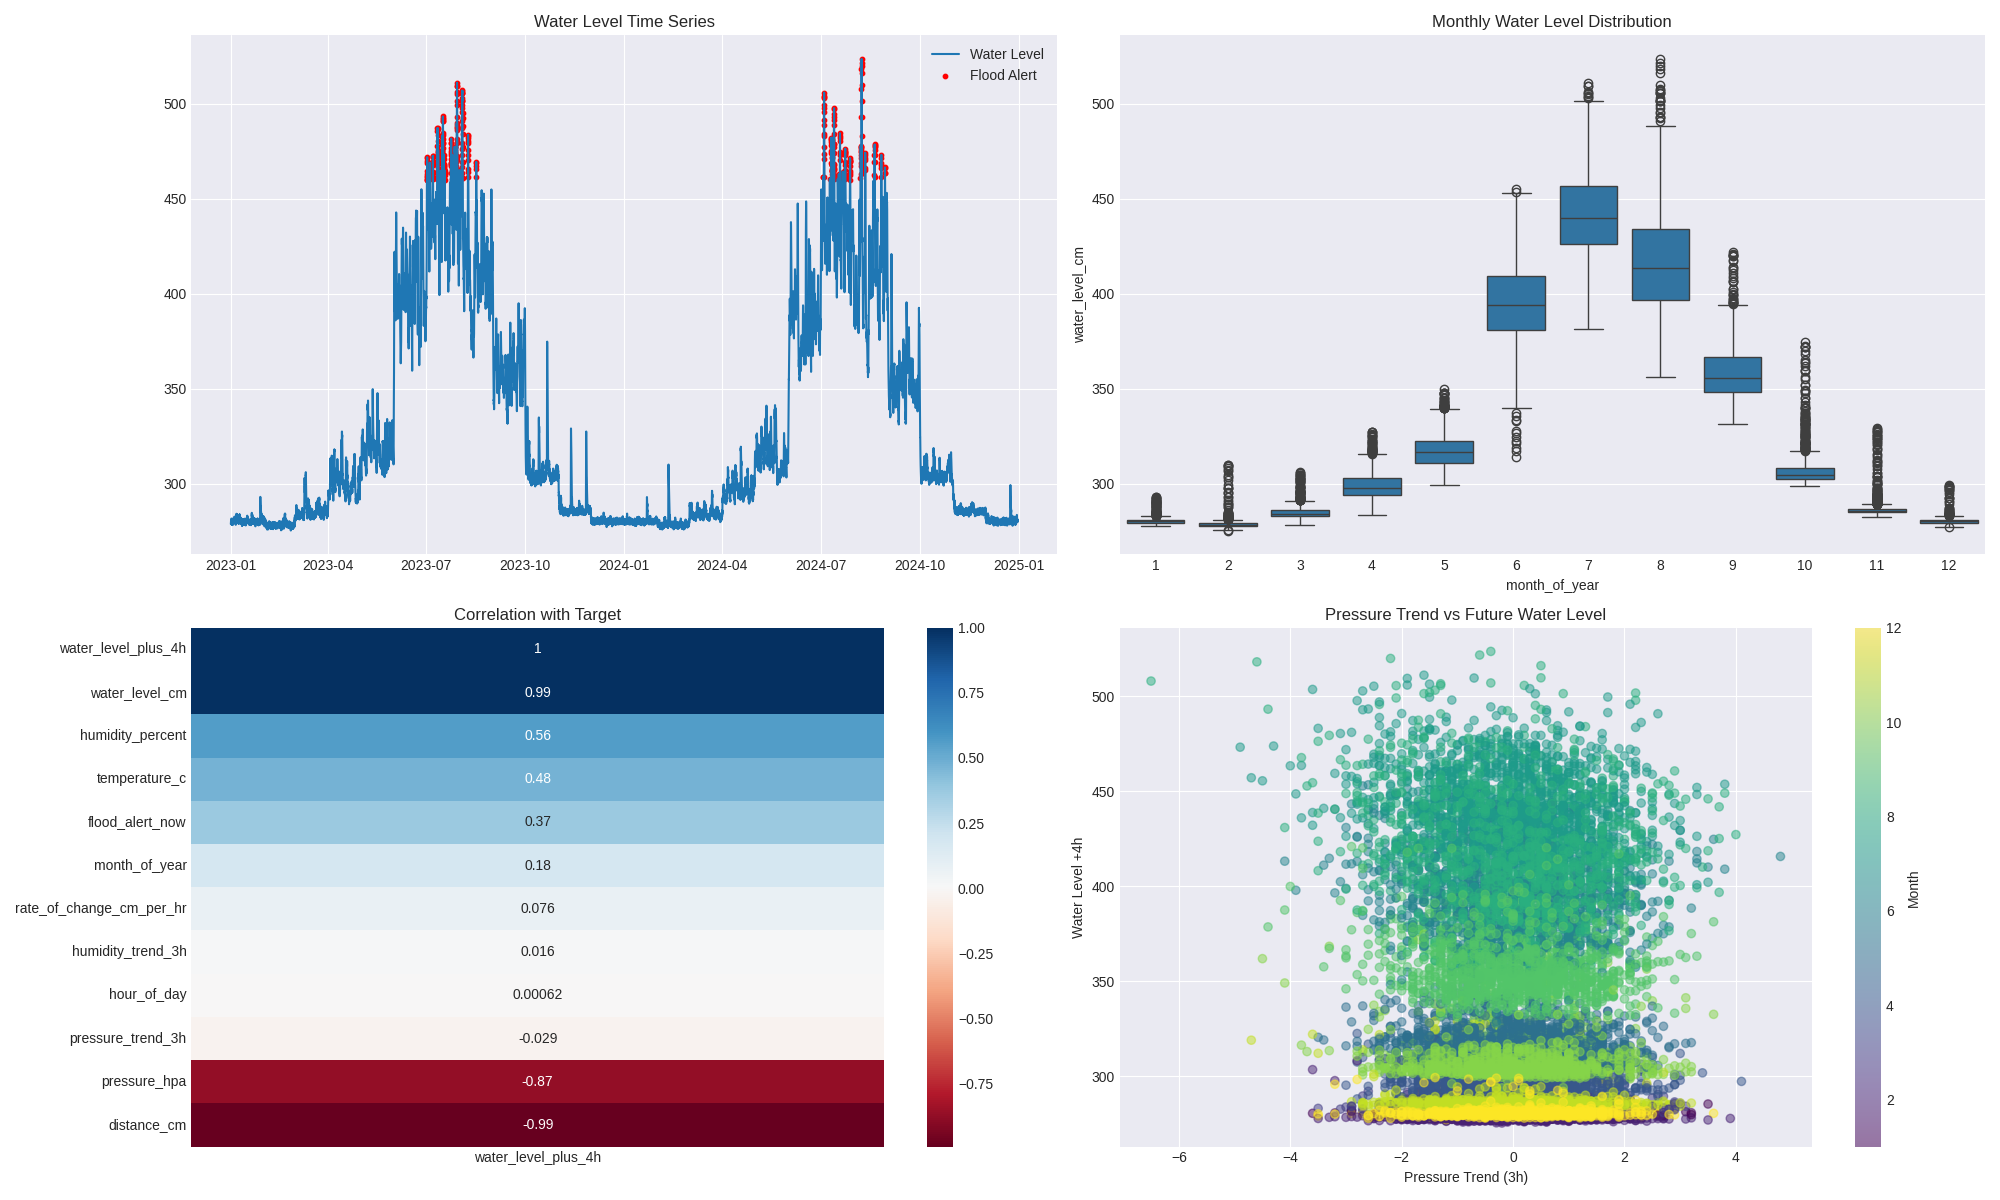
\includegraphics[width=\textwidth,height=0.7\textheight,keepaspectratio]{../Model/flood_plots/eda_plots.png}
    \end{column}
  \end{columns}
\end{frame}

\begin{frame}{TFJS Conversion \& Inference Pipeline}
  \begin{itemize}
    \item \texttt{.h5} model converted to \texttt{model.json} and \texttt{.bin} weights using \texttt{tensorflowjs\_converter}.
    \item Deployed to \texttt{/public} directory of the Next.js app.
    \item \textbf{Browser Inference:} \texttt{loadModel()} fetches weights and registers the custom Attention Layer.
    \item Dashboard intercepts last 48 readings, engineers features on-the-fly, and runs prediction.
    \item Inference time is $< 100$ms on the client device.
  \end{itemize}
\end{frame}

\begin{frame}{ML Diagnostics Panel}
  \begin{itemize}
    \item Available to Admin users on the Predictions page.
    \item Shows active model status, tensor shapes, and live latency.
    \item Displays Feature Contribution breakdown (which sensor is driving the current prediction).
    \item Provides confidence intervals for the 4-hour forecast.
  \end{itemize}
\end{frame}

\section{Experimental Results \& Limitations}

\begin{frame}{System Performance Results}
  \begin{itemize}
    \item \textbf{Latency:} End-to-end data latency (Sensor $\rightarrow$ ThingSpeak $\rightarrow$ Dashboard) is approx. 1-2 seconds.
    \item \textbf{Load Time:} First Contentful Paint $< 1.5$s via Vercel Edge Network.
    \item \textbf{ML Accuracy:} Training Mean Absolute Error (MAE) of 3.42 cm.
    \item \textbf{Reliability:} Backend request coalescing successfully prevents ThingSpeak rate limits (15s minimum) even with 100+ concurrent dashboard users.
  \end{itemize}
\end{frame}

\begin{frame}{Alerting \& UX Results}
  \begin{itemize}
    \item Cooldown timers effectively prevent alert spam (e.g., only one RAPID\_WATER\_RISE alert per minute).
    \item Glassmorphism UI maintained stable 60 FPS during animations.
    \item PWA Service Worker successfully cached the application shell, allowing the app to open instantly offline.
  \end{itemize}
\end{frame}

\begin{frame}{Limitations: Hardware}
  \begin{itemize}
    \item \textbf{Power Dependency:} The ESP32 requires continuous power; no solar/battery fallback implemented yet.
    \item \textbf{Connectivity:} Relies on Wi-Fi. Unsuitable for remote rivers without GSM/LoRa infrastructure.
    \item \textbf{Sensor Range:} HC-SR04 ultrasonic sensor has a limited maximum range ($\sim$400cm) and can be affected by heavy rain or debris.
  \end{itemize}
\end{frame}

\begin{frame}{Limitations: Software \& ML}
  \begin{itemize}
    \item \textbf{Cold Start:} ML model requires 48 historical data points. Currently mitigated by padding with static sample data.
    \item \textbf{ThingSpeak Limits:} Free tier restricts updates to every 15 seconds.
    \item \textbf{Model Generalisation:} Trained specifically on Assam flood data; requires re-training for rivers with different topographical characteristics.
  \end{itemize}
\end{frame}

\section{Conclusion \& Future Scope}

\begin{frame}{Conclusion}
  \begin{itemize}
    \item FloodEye successfully demonstrates a low-cost, full-stack IoT solution for flood monitoring.
    \item The integration of edge hardware (ESP32) with a modern web frontend (Next.js) provides an accessible early warning system.
    \item In-browser Machine Learning (TensorFlow.js) proves to be a viable, zero-server-cost architecture for real-time predictive analytics.
    \item The system fulfills its primary objective of delivering actionable, micro-local hydrological data.
  \end{itemize}
\end{frame}

\begin{frame}{Future Scope: Hardware Upgrades}
  \begin{itemize}
    \item Transition from Wi-Fi to \textbf{LoRaWAN} or GSM (SIM800L) for remote deployments.
    \item Replace HC-SR04 with industrial-grade waterproof LiDAR or radar sensors for better accuracy in heavy rain.
    \item Implement Solar + Li-Po battery management system for autonomous off-grid operation.
  \end{itemize}
\end{frame}

\begin{frame}{Future Scope: Software Upgrades}
  \begin{itemize}
    \item Implement full PostgreSQL database (Neon) to bypass ThingSpeak's 15-second limitation and store unlimited history.
    \item Introduce user authentication (NextAuth) for public accounts to subscribe to specific SMS alerts (Twilio integration).
    \item Expand the ML model to include external weather API forecasts (e.g., OpenWeatherMap rainfall data) as additional input features.
  \end{itemize}
\end{frame}

\begin{frame}
  \centering
  \Huge \textbf{Thank You}
  
  \vspace{1cm}
  \Large Questions \& Answers
\end{frame}

\end{document}
